% SIAM Article Template
\documentclass[hidelinks,onefignum,onetabnum]{siamart220329}

% Information that is shared between the article and the supplement
% (title and author information, macros, packages, etc.) goes into
% ex_shared.tex. If there is no supplement, this file can be included
% directly.

% SIAM Shared Information Template
% This is information that is shared between the main document and any
% supplement. If no supplement is required, then this information can
% be included directly in the main document.


% Packages and macros go here
\usepackage{lipsum}
\usepackage{amsfonts}
\usepackage{graphicx}
\usepackage{epstopdf}
\usepackage{algorithmic}
\usepackage{physics}
\usepackage{bm}
\ifpdf
  \DeclareGraphicsExtensions{.eps,.pdf,.png,.jpg}
\else
  \DeclareGraphicsExtensions{.eps}
\fi

% Add a serial/Oxford comma by default.
\newcommand{\creflastconjunction}{, and~}

% Used for creating new theorem and remark environments
\newsiamremark{remark}{Remark}
\newsiamremark{hypothesis}{Hypothesis}
\crefname{hypothesis}{Hypothesis}{Hypotheses}
\newsiamthm{claim}{Claim}

% Sets running headers as well as PDF title and authors
\headers{18.336 Final Report}{L. Van Mu\~noz}

% Title. If the supplement option is on, then "Supplementary Material"
% is automatically inserted before the title.
\title{18.336 Final Report}

% Authors: full names plus addresses.
\author{Lorenzo Van Mu\~noz\thanks{Department of Physics, Massachusetts Institute
of Technology, 77 Massachusetts Avenue, Cambridge, MA 02139
  (\email{lxvm@mit.edu}, \url{http://web.mit.edu/lxvm/www/}).}
}

\usepackage{amsopn}
\DeclareMathOperator{\diag}{diag}


%%% Local Variables: 
%%% mode:latex
%%% TeX-master: "ex_article"
%%% End: 


% Optional PDF information
\ifpdf
\hypersetup{
  pdftitle={18.336 Final Project},
  pdfauthor={Lorenzo Van Munoz}
}
\fi

% The next statement enables references to information in the
% supplement. See the xr-hyperref package for details.

% \externaldocument[][nocite]{ex_supplement}

% FundRef data to be entered by SIAM
%<funding-group specific-use="FundRef">
%<award-group>
%<funding-source>
%<named-content content-type="funder-name"> 
%</named-content> 
%<named-content content-type="funder-identifier"> 
%</named-content>
%</funding-source>
%<award-id> </award-id>
%</award-group>
%</funding-group>

\begin{document}

\maketitle

\section{Introduction}
In optics, the design of metamaterials is blurring the line between the
traditions of geometric optics and diffractive optics by allowing the fine
tuning of optical elements at a sub-wavelength scale. Often, the inverse design
problem poses a huge computational challenge due to the demanding nature of
full-wave simulations in 3D on large structures. As an alternative to full-3D
simulations, metamaterials which are thin compared to the wavelengths of light
incident upon them can be approximated by metasurfaces which have impedance data
parametrized on a surface \cite{kuesterAveragedTransitionConditions2003}. In
this report I explore a fast and accurate boundary integral method that is
only applicable to planar, 2D periodic metasurfaces with periodic boundary data
and employs Fourier pseudospectral acceleration.

\section{Problem formulation}

The metasurface scattering problem considers a geometry of two half-spaces,
$\Omega_1, \Omega_2$, separated by a plane $\Gamma$ and tries to solve for the
total electromagnetic fields given an incident planewave with wavenumber $k$. In
the half spaces, the fields must satisfy Maxwell's curl equations:
\begin{align}
  -\mu \partial_t \bm{H} &= \curl \bm{E} \\
  \epsilon \partial_t \bm{E} &= \curl \bm{H}
\end{align}
and on the plane, the fields must satisfy a local jump condition created by the
metasurface's impedance parameters $Z_e = Y_e^{-1}$ and $Z_m = Y_m^{-1}$:
\begin{align}
  \hat{\bm{n}} \times \qty(\bm{H}_2 - \bm{H}_1) &= \frac{1}{2} Y_{e} \qty(\bm{E}_2 + \bm{E}_1) \\
  -\hat{\bm{n}} \times \qty(\bm{E}_2 - \bm{E}_1) &= \frac{1}{2} Y_{m} \qty(\bm{H}_2 + \bm{H}_1).
\end{align}
In the equations above, $\hat{\bm{n}}$ is the normal vector to $\Gamma$ and the
subscripts on the fields denote the limiting value of that field in the
specified half-space as it approaches the given point in $\Gamma$. These jump
conditions on the tangential fields were first formulated in
\cite{kuesterAveragedTransitionConditions2003} as an effective medium
description of thin scatterers such as flat antennae.

\subsection{Boundary conditions}
Beyond the jump conditions, the solution must also satisfy a radiation condition
in the half-spaces that the fields must have uniformly-convergent Rayleigh-Bloch
expansions as planewaves away from $\Gamma$
\cite{barnettNewIntegralRepresentation2011}.

Moreover, I restrict to the case that the metamaterial parameters, $Y_e, Y_m$,
are periodic in two-dimensions. Namely, they satisfy $Y(x+nL_x, y+mL_y) =
Y(x,y)$ for all $(x,y) \in \bm{R}^2$ given periods $L_x, L_y$. Lastly, the third
dimension, $z$, is referred to as the scattering axis, and thus $\hat{\bm{n}} =
\hat{\bm{z}}$.

\subsection{Reduction to 2D}
When simplifying the problem to 2D, I assume that the metasurface parameters are
invariant in $y$ so that all of their $y$ derivatives vanish. In this setting,
Maxwell's equations decouple into two independent equations for the
transverse-electric (TE) and transverse-magnetic (TM) modes, which are governed
by the solution to $H_z$ and $E_z$. It can be derived that the PDEs for either
mode reduce to the following Helmholtz problem in the half-planes
\cite{perez-arancibiaSidewaysAdiabaticityRay2018}
\begin{align}
  \nabla^2 u + k^2 u = 0
\end{align}
and the jump conditions on the curve
\begin{align}
\partial_z \qty(u_2 - u_1) &= -ik\alpha \qty(u_2 + u_1) \\
\partial_z \qty(u_2 + u_1) &= -ik\beta  \qty(u_2 - u_1).
\end{align}
Above we have introduced modified metasurface parameters $\alpha$ and $\beta$
which are $L$-periodic and can be related back to the original parameters. The
exact form depends on whether the problem is formulated for the TE or TM mode,
and is not essential for the solution methods for the PDE.

\subsection{Quasi-periodic Green's function}
The exact solution of the problem can be obtained with a properly-formulated
Green's function for the 2D PDE, $G(\bm{r}, \bm{r}')$, for a point source at
$\bm{r}=(x,z)$ and a target point $\bm{r}' = (x', y')$. In the half planes, for
$\bm{r} \in \Omega_1 \cup \Omega_2$, the Green's function must satisfy
\begin{align}
  \nabla^2_{\bm{r}} G(\bm{r}, \bm{r}') + k^2 G(\bm{r}, \bm{r}') = -\delta(\bm{r} - \bm{r}')
\end{align}
and on the metasurface, for $\bm{r} \in \Gamma$, the condition is
\begin{align}
  \partial_z \qty(G_2(\bm{r}, \bm{r}') - G_1(\bm{r}, \bm{r}')) &= -ik\alpha \qty(G_2(\bm{r}, \bm{r}') + G_1(\bm{r}, \bm{r}')) \\
  \partial_z \qty(G_2(\bm{r}, \bm{r}') + G_1(\bm{r}, \bm{r}')) &= -ik\beta  \qty(G_2(\bm{r}, \bm{r}') - G_1(\bm{r}, \bm{r}')).
\end{align}
In particular, the exact Green's function, $G_{QP}$, can be obtained from the free-space 2D
Green's function, $G_0(\bm{r}, \bm{r}')$, given by
\begin{align}
  G_0(\bm{r}, \bm{r}') = \frac{i}{4} H_0^{(1)}(k\abs{\bm{r} - \bm{r}'})
\end{align}
where $H_0^{(1)}$ is a zero-th order Hankel function of the first kind. While
$G_0$ satisfies the radiation condition, the periodicity can be achieved 
by summing phased copies on the periodic lattice of unit cells to obtain a
quasi-periodic Green's function. This becomes
\begin{align}
  G_{QP}(\bm{r}, \bm{r}') = \frac{i}{4} \sum_{n=-\infty}^{\infty} e^{ik\cos(\theta)nL} H_0^{(1)}(k\sqrt{(x-x'+nL)^2 + (y-y')^2})
\end{align}
where $\theta$ is the angle of incidence measured from the $\hat{\bm{x}}$ axis
\cite{barnettNewIntegralRepresentation2011}.

Numerical evaluation of the infinite sum in the quasi-periodic Green's function
has received much attention and can be evaluated by methods such as Ewald
summation and summation with a window function. Due to its simplicity, I
implemented a windowed sum, which takes the following form:
\begin{align}
  G_{QP}^{A}(\bm{r}, \bm{r}') = \frac{i}{4} \sum_{n=-\infty}^{\infty} w_A(x-x'+nL) e^{ik\cos(\theta)nL} H_0^{(1)}(k\sqrt{(x-x'+nL)^2 + (y-y')^2})
\end{align}
with the window function, $w_A$, defined by
\begin{align}
  w_A(x; x_0, x_1) = \begin{cases}
    0 & \text{if }\abs{x} \leq x_0 \\
    \exp(2\exp(1/u)/(1-u)) & \text{if }x_0 < \abs{x} < 1, u = (\abs{x}-x_0)/(x_1-x_0)\\
    1 & \text{if }\abs{x} \geq x1
  \end{cases}
\end{align}
It is known that integrals of periodic functions times the windowed Green's
function converge superalgebraically with respect to the window size $A$
\cite{brunoWindowedGreenFunction2016}.

Note that the quasi-periodic Green's function is ill-defined at points where
$(k\cos(\theta) + nL)^2 = k^2$ for any integer $n$. This can be shown by
applying the Poisson summation formula to $G_{QP}$. Such a point is called a
Wood anomaly.

\subsection{Integral formulation}
We can solve the PDE as a boundary integral by using the Green's function and
making the ansatz
\begin{align}
  u_i(\bm{r}) = \int_{\Gamma} G_{QP}(\bm{r}, \bm{r}') \sigma_i(\bm{r}') d\bm{r}'.
\end{align}
We equivalently write this as a single-layer operator, $u_i = S[\sigma_i]$.
Then the jump conditions become 
\cite{coltonInverseAcousticElectromagnetic2013}
\begin{align}
  u_2 + u_1 &= S[\sigma_2 + \sigma_1] \\
  u_2 - u_1 &= S[\sigma_2 - \sigma_1] \\
  \partial_z \qty(u_2 + u_1) &= -\frac{1}{2}\qty(\sigma_2 - \sigma_1) \\
  \partial_z \qty(u_2 - u_1) &= -\frac{1}{2}\qty(\sigma_2 + \sigma_1)
\end{align}
and by introducing new variables $\xi_1 = \sigma_1 + \sigma_2, \xi_2 = \sigma_1
- \sigma_2$ we use the jump conditions to arrive at the following system of
boundary integral equations
\begin{align}
(-I/2 + ik\alpha(x) S)\xi_1 &= -2ik\alpha(x) e^{ik\cos(\theta)x} \\
(-I/2 + ik\beta(x)  S)\xi_2 &= -2i\sqrt{k^2 - (k\cos(\theta))^2}e^{ik\cos(\theta)x}.
\end{align}
This integral formulation was derived by Carlos P\'erez-Arancibia in an ongoing
collaboration. Since these are integral equations of the second kind, they are
favorable for iterative methods.

\section{Spectrally accurate quadrature for closed boundaries}

The Kress quadrature rule (originally due to Martensen and Kussmaul) was
originally invented as a specialized quadrature for the single-layer operator
with a logarithmic kernel, such as for $G_{QP}$. On closed curves, this method
converges spectrally and faster than other quadratures, and is not FMM
compatible since the quadrature rule globally modifies the kernel
\cite{haoHighorderAccurateNystrom2012}. In this work, a notable difference is
that we are performing an integral over an open curve, and as a result care must
be taken to evaluate the kernel appropriately. In particular, a main difference
I encountered in this work is that the quantity $x-x'$ can be evaluated directly
for closed curves, but for open curves must be taken to be the minimum distances
of $x-x'$ for all periodic images of $x$ and $x'$.

\subsection{Singularity separation}
The Kress quadrature rule requires knowledge of the kernel, $K(x, x')$, and in
particular a decomposition of the form $K(x, x') =
K_1(x,x')\log(4\sin[2](\frac{x-x'}{2})) + K_2(x, x')$, where $K_1$ and $K_2$ are
analytic and $2\pi$ periodic \cite{coltonInverseAcousticElectromagnetic2013}. In
particular, for the 2D free space Green's function, $G_0$, such a decomposition
is known
\begin{align}
  G_0(x,x') = \begin{cases}
    -\frac{1}{4\pi}J_0(k\abs{x-x'})\log(4\sin[2](\frac{x-x'}{2})) + \frac{i}{4}H_0^{(1)}(k\abs{x-x'}) & \text{if }x \neq x' \\
    -\frac{1}{4\pi}J_0(k\abs{x-x'})\log(4\sin[2](\frac{x-x'}{2})) + \qty(\frac{i}{2} - \frac{\gamma}{2\pi} - \frac{1}{2\pi}\log(\frac{k}{2})) & \text{if }x = x'
  \end{cases}
\end{align}
In the derivative above we assumed that $\Gamma$ is a unit-speed parameterized
curve of length $2\pi$ and used the Euler-Mascheroni constant $\gamma$.

To extend this decomposition to $G_{QP}$, note that the evaluation points can
always be chosen around a single singularity of the quasi-periodic kernel,
namely $x-x'=0$, although there are singularities at all $x-x'=0 \mod 2\pi$. The
terms with $n\neq0$ in the quasi-periodic sum can be evaluated regularly with
the correction above applied only to the $n=0$ term. However, a major limitation
of the Kress quadrature on $G_{QP}$ is that the remaining terms in the sum are
not truly a periodic function unless $k\cos(\theta)L = 0 \mod 2\pi$, which
corresponds to having the incident wave be exactly a Bloch mode providing
periodic boundary data. Other projects may want to investigate if a singularity
separation which does not distinguish $n=0$ in the $G_{QP}$ sum is available.

\subsection{Nystr\"om discretization}
To discretize the single-layer operator we employ the following quadrature
\cite{haoHighorderAccurateNystrom2012}
\begin{align}
  \label{eq:quad}
  \int_0^{2\pi} K(x,x')\sigma(x')dx' \approx \sum_{j=1}^{2N} R_j^{(N)}(x) K_1(x,x_j) \sigma(x_j) + \frac{\pi}{N} \sum_{j=1}^{2N} K_2(x,x_j) \sigma(x_j)
\end{align}
where the quadrature nodes are chosen on an equispaced grid $x_j = j\pi/N$ and
the weights $R_j^{(N)}(x)$ are given by
\begin{align}
  R_j^{(N)}(x) = -\frac{2\pi}{N}\qty(\sum_{m=1}^{N-1} \frac{\cos(m(x_j-x))}{m} + \frac{\cos(N(x_j-x))}{2N}).
\end{align}
The target points can be chosen freely, but as will be explained below it is
fastest to choose them to be on the same points as the quadrature grid.

\section{Fast iterative solver}

To convert the preceding quadrature into a fast method, it suffices to apply the
second-kind Fredholm integral operator as a fast matrix-vector product, which
can then be used in a general purpose iterative solver such as GMRES. This
acceleration becomes increasingly important when dealing with small wavenumbers
or rapidly-varying metasurface parameters that require finer discretizations of
the boundary to resolve the solution. The main observation that will allow us to
develop a fast method is that the discretization of $S$ evaluated on equispaced
nodes is a circulant matrix. This can be seen in \eqref{eq:quad} by noticing
that when the source and target points are the same equispaced grid, the weights
become a circulant matrix, and the distances, $\abs{x_i - x_j}$, when interpreted
in a periodic fashion are also circulant.


\subsection{Fourier pseudospectral matrix-vector product}

When $S$ is a circulant matrix, denote one of its columns by $s$ and observe
that the product $S\xi$ is equal to the circular convolution $s \star \xi$. In
Fourier space, this operation is equivalent to point-wise multiplication, i.e.
$\widehat{s \star \xi} = \hat{s} \hat{\xi}$. Let $\mathcal{F}$ denote the
discrete Fourier transform matrix. The fast matrix-vector product is given by
\begin{align}
  (-I/2 + ik\alpha(x)S) = \mathcal{F}^{-1} (-I/2 + ik\mathcal{F} \alpha(x) \mathcal{F}^{-1} \hat{s}) \mathcal{F}.
\end{align}
Compared to a direct solver with $\mathcal{O}(N^3)$ complexity, this
matrix-vector product is a $\mathcal{O}(N\log(N))$ operation whose complexity
stays the same if GMRES converges in a fixed number of operations, giving a fast
method for the solution of the auxiliary densities $\xi_1, \xi_2$ and thus the
surface densities $\sigma_1, \sigma_2$.

\section{Results}

In this section I present results for a single metasurface and compare the
convergence and timings of both fast and direct solvers.

\subsection{Problem parameters}

The metasurface illustrated in Fig. \ref{fig:parameters} was shown in
\cite{perez-arancibiaSidewaysAdiabaticityRay2018} to deflect an incident wave of
wavenumber $k$ at angle $\theta_i$ to another wave at angle $\theta_t$.
The analytic form of the metasurface parameters is
\begin{align}
  \alpha(x) &= -\sin(\theta_i) \qty(1 + e^{ikd}) \\
  \beta(x) &= -\sin(\theta_i) \qty(1 - e^{ikd})
\end{align}
where $d = \cos(\theta_t) - \cos(\theta_i)$ and the metasurface period is $L =
2\pi/k\abs{d}$. In the calculations that follow, I take $k=10, \theta_i =
-\pi/2, \theta_t=-\pi/6$. This corresponds to deflecting a normally incident
wave by 60 degrees. The calculation could be more difficult with more quickly
varying metasurface parameters or with a more oblique $\theta_i$ that is still a
Bloch mode for the given wavenumber, but this mild parameter choice is good for
validation.

In Fig. \ref{fig:solution} are solutions for the surface densities and fields
for the specified problem. They display the same periodicity that exists in
metasurface and boundary data, although they are more rapidly varying.

\begin{figure*}
  \centering
  \includegraphics[height=3.5cm]{true_sol.png}
  \hspace{1cm}
  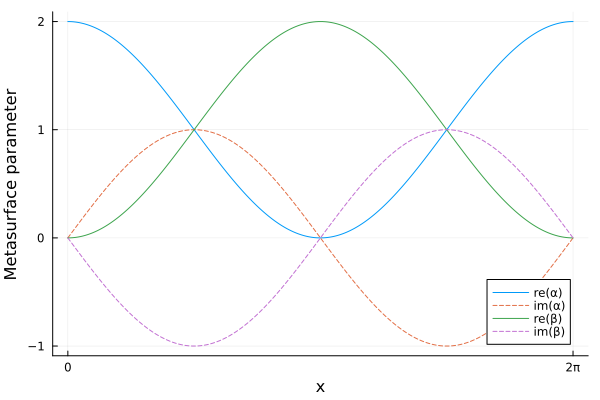
\includegraphics[height=3.5cm]{params.png}
  \caption{Representative geometry of the 2D metasurface scattering problem and
  parameters of a metasurface which deflects an incident planewave to an
  outgoing planewave with a new wavevector. This metasurface only accomplishes
  its goal for a single wavenumber and a single set of incident and outgoing
  wavevectors. Leftmost figure was taken from
  \cite{perez-arancibiaSidewaysAdiabaticityRay2018}. Generally the periodic
  metasurface, which acts as a diffraction grating, can only couple Bloch
  wavevectors on either side of the surface.}
  \label{fig:parameters}
\end{figure*}


\begin{figure*}
  \centering
  \includegraphics[height=3.5cm]{densities.png}
  \includegraphics[height=3.5cm]{fields.png}
  \caption{Solutions of the deflecting metasurface scattering problem with
  parameters $k=10, \theta_i=-\pi/2, \theta_t=-\pi/6$. The line plot displays
  the real and imaginary parts of the surface current densitites above and below
  the metasurface as obtained by the solver. The heatmap displays the real part
  of the fields, which clearly depict the normally-incident planewave from above
  the sheet being deflected to an obliquely-outgoing planewave.}
  \label{fig:solution}
\end{figure*}

\subsection{Convergence tests}

Fig. \ref{fig:converge} presents self-convergence results for the direct solver,
and the results are identical for the fast solver. Unlike Kress quadrature on a
closed surface, the rate of convergence is only analytic in this problem with an
open surface. Still, the solution converges rapidly with 4th order convergence,
giving a practical solver that converges in a modest number of grid points.
Possibilities of why the convergence is not spectral include bugs as well as an
imperfect singularity cancellation in the Kress quadrature for $G_{QP}$, which
may be sensitive to the windowed sum. Taking more difficult metasurface or
scattering parameters may also slow the rate of convergence.

\begin{figure*}
  \centering
  \includegraphics[height=3.5cm]{densities_conv_direct.png}
  \includegraphics[height=3.5cm]{fields_conv_direct.png}
  \caption{The spectrally-accurate Kress quadrature rule used in this report
  appears to only yield algebraic convergence in the solution of the surface
  current densities and the fields, which were evaluated at a distance of one
  wavelength away from the metasurface. In fact, this is due to treatment of the
  quasi-periodic Green's function, which is windowed and thus not truly
  periodic, and moreover, is only corrected with the Kress quadrature rule at
  one of the singularities, therefore breaking the periodicity. Nonetheless, the
  rate of algebraic convergence that can be seen in the surface density plots is
  $\mathcal{O}(N^{-4})$ and is sufficiently rapid to obtain 10 digits of
  accuracy when requesting $N=128$.}
  \label{fig:converge}
\end{figure*}

\subsection{Method scaling}

Fig. \ref{fig:scaling} present the scaling of the direct solver,
$\mathcal{O}(N^3)$ versus the fast solver, $\mathcal{O}(N\log(N))$. The
implementations are both in very good agreement with the asymptotic scalings for
$N>100$.

\begin{figure*}
  \centering
  \includegraphics[height=3.5cm]{scaling.png}
  \caption{Wall clock time versus $N$ comparing the direct solver and fast
  solver for calculating the surface densities of the deflecting metasurface
  with parameters $k=10, \theta_i = -\pi/2, \theta_t = -\pi/6$. All calculations
  were performed on a single core of an Intel i5-12500 processor, and they
  include the time to evaluate the boundary data, construct the single-layer
  operator, and solve the linear system. The only cached data used were the
  Kress quadrature weights and FFTW plans.}
  \label{fig:scaling}
\end{figure*}

In summary, Table \ref{tab:summary} presents timings and errors for the Kress
quadrature with direct and fast methods. The crossover of the fast method over
the direct solver is apparent at $N=32$, where the relative error is already at
the 8th significant digit. Clearly while high-order methods converge quickly
enough to not need many grid points, the fast method has a small enough constant
to make it competitive in most cases.

\begin{table}
  \centering
  \begin{tabular}{|c|c|c|c|}
    \hline
    N & Direct timing (s) & Fast timing (s) & Relative error \\ \hline
    $2^5$ & 0.00019 & 0.00017 & 5.4e--08 \\
    $2^7$ & 0.00297 & 0.00060 & 2.1e--10 \\
    $2^9$ & 0.11071 & 0.00222 & 8.2e--13 \\
    $2^{11}$ & 6.33158 & 0.00944 & 5.1e--15 \\ \hline
  \end{tabular}
  \caption{Representative timings and relative errors taken from the preceding
  plots comparing the speed of the two solvers and the relative error in the
  surface density of their solution. The relative error displayed is the maximum
  relative error of either the surface density above or below the sheet.}
  \label{tab:summary}
\end{table}

\subsection{Code availability}

The implementation of the direct and fast solvers is available at the following
repository \url{https://github.com/lxvm/MetaBIE.git}. Generating the data,
figures, and report is as simple as running a shell script and takes about ten
minutes.

\section{Discussion}
The most interesting result of this work has been to discover that the
convergence of the Kress quadrature in this case with an open boundary is only
algebraic with 4th order convergence. Although I can't rule out the possibility
of a bug, a more careful analysis of the singularity separation for $G_{QP}$ may
be able to reveal the origin of the algebraic rate.
Further investigation also is necessary to determine whether the boundary integral
formulation of the full 3D problem still reduces to either a circulant or
block-circulant representation that is compatible with the Fourier
pseudospectral method employed in this report. Additionally, it would be
worthwhile to pursue other quadrature rules which can recover spectral
convergence in the presence of both periodic and quasi-periodic boundary data
while also being accelerated by either the method in this report or an FMM,
which would have to use a potential expansion tailored to the quasi-periodic
Green's function. In my previous research, I have developed a Fourier spectral
method solver for the 3D problem, which also obtains $\mathcal{O}(N\log(N))$
complexity if solved using iterative method, and believe that it should be the
easiest path to a fast 3D solver if I can resolve some numerical conditioning
issues that arise in the method.

\bibliographystyle{siamplain}
\bibliography{references}
\end{document}
